\documentclass[11pt]{article}

\usepackage[a4paper]{geometry}
\geometry{left=2.0cm,right=2.0cm,top=2.5cm,bottom=2.5cm}

% Chinese support
\usepackage{ctex}

% Math packages
\usepackage{amsmath,amsfonts,amssymb,amsthm,bm,mathrsfs,mathtools,breqn}

% Graphics and Colors
\usepackage{graphicx}
\usepackage{xcolor}
\usepackage{tikz}
\usetikzlibrary{arrows.meta,positioning}
\usepackage{pgfplots}
\pgfplotsset{compat=1.18}
\usepackage{circuitikz}
\graphicspath{{fig/}}

% Units
\usepackage{siunitx}

% Algorithms
\usepackage{algorithm}
\usepackage[noend]{algpseudocode}

% Layout and formatting
\usepackage{fancyhdr}
\usepackage[framemethod=TikZ]{mdframed}
\usepackage{fontspec}
\usepackage{fontsize}
\usepackage{adjustbox}
\usepackage{float}
\usepackage{multicol}
\usepackage{multirow}
\usepackage{pdfpages}
\usepackage{wrapfig}
\usepackage{subcaption}
\usepackage[inline]{enumitem}

% Tables
\usepackage{booktabs}
\usepackage{bigstrut,rotating}

% Listings
\RequirePackage{listings}

% Hyperlinks
\usepackage{hyperref}
\hypersetup{colorlinks=true,linkcolor=blue}

% Cross-referencing
\usepackage[capitalize]{cleveref}
\Crefname{section}{Section}{Sections}
\Crefname{table}{Table}{Tables}
\crefname{table}{Table.}{Tabs.}

% Listing settings
\definecolor{dkgreen}{rgb}{0,0.6,0}
\definecolor{gray}{rgb}{0.5,0.5,0.5}
\definecolor{mauve}{rgb}{0.58,0,0.82}

\lstset{
  frame=tb,
  aboveskip=3mm,
  belowskip=3mm,
  showstringspaces=false,
  columns=flexible,
  framerule=1pt,
  rulecolor=\color{gray!35},
  backgroundcolor=\color{gray!5},
  basicstyle={\small\ttfamily},
  numbers=none,
  numberstyle=\tiny\color{gray},
  keywordstyle=\color{blue},
  commentstyle=\color{dkgreen},
  stringstyle=\color{mauve},
  breaklines=true,
  breakatwhitespace=true,
  tabsize=3,
}

\setmainfont{Palatino Linotype}
\setCJKmainfont{SimSun}[BoldFont=SimHei, ItalicFont=KaiTi]
\setCJKsansfont{SimHei}
\setCJKmonofont{FangSong}
\punctstyle{kaiming}
% 偏好的几个字体, 可以根据需要自行加入字体ttf文件并调用

% Restore standard emphasis to avoid requiring an undefined environment (kaishu).
% The original redefinition used an environment `kaishu` which is not defined
% in a default ctex setup and causes compilation errors. Use \textit for
% emphasis which works across engines.
\renewcommand{\emph}[1]{\textit{#1}}

%改这里可以修改实验报告表头的信息
\newcommand{\experiName}{弦上驻波实验}
\newcommand{\supervisor}{王佳怡}
\newcommand{\name}{邓思豪}
\newcommand{\studentNum}{2023K8009909008}
\newcommand{\class}{3}
\newcommand{\group}{01}
\newcommand{\seat}{5}
\newcommand{\dateYear}{2026}
\newcommand{\dateMonth}{1}
\newcommand{\dateDay}{7}
\newcommand{\room}{西实204}
\newcommand{\others}{$\square$}


\begin{document}



\begin{center}
    \LARGE \bf 《\, 基\, 础\, 物\, 理\, 实\, 验\, 》\, 实\, 验\, 报\, 告
\end{center}

\begin{center}
    \noindent \emph{实验名称}\underline{\makebox[25em][c]{\experiName}}
    \emph{指导教师}\underline{\makebox[8em][c]{\supervisor}}\\
    \emph{姓名}\underline{\makebox[6em][c]{\name}} 
    % 如果名字比较长, 可以修改box的长度"6em"
    \emph{学号}\underline{\makebox[10em][c]{\studentNum}}
    \emph{分班分组及座号} \underline{\makebox[5em][c]{\class \ -\ \group \ -\ \seat }\emph{号}} （\emph{例}:\, 1\,-\,04\,-\,5\emph{号}）\\
    \emph{实验日期} \underline{\makebox[3em][c]{\dateYear}}\emph{年}
    \underline{\makebox[2em][c]{\dateMonth}}\emph{月}
    \underline{\makebox[2em][c]{\dateDay}}\emph{日}
    \emph{实验地点}\underline{{\makebox[6em][c]\room}}
    \emph{调课/补课} \underline{\makebox[3em][c]{\others\ 是}}
    \emph{成绩评定} \underline{\hspace{5em}}
    {\noindent}
    \rule[8pt]{17cm}{0.2em}
\end{center}

\part{弦上驻波实验}



\section{实验目的}
\begin{enumerate}
    \item 观察在两端固定的弦线上形成的驻波现象，了解弦线达到共振和形成稳定驻波的条件；
    \item 测定弦线上横波的传播速度；
    \item 用实验的方法确定弦线作受迫振动时共振频率与半波长个数 $n$、弦线有效长度、张力及弦密度之间的关系；
    \item 用对数作图和最小二乘法对共振频率与张力关系的实验结果作线性拟合，处理数据，并给出结论。
\end{enumerate}

\section{实验原理}

\subsection{驻波的理论基础}

\begin{figure}[H]
    \centering
    
\includegraphics[width=0.8\textwidth]{fig1}
    \caption{某时刻的入射波 E(r)}
    \label{fig:fig1}
\end{figure}

驻波由频率和振幅均相同、振动方向一致、传播方向相反的两列波叠加而来。一般地，设两列方向相反的波的方程分别为：
\begin{equation}
    y_{1}=A \cos(\omega t-kx+\varphi_{1})
\end{equation}
\begin{equation}
    y_{2}=A \cos(\omega t+kx+\varphi_{2})
\end{equation}
其中，$k=\frac{2\pi}{\lambda}$ 为角波数，$\lambda$ 是波长。当两列波合成时有：
\begin{equation}
    y_{1}+y_{2}=2A \cos(kx+\frac{\varphi_{2}-\varphi_{1}}{2})\cos(\omega t+\frac{\varphi_{1}+\varphi_{2}}{2})
\end{equation}
由式(3)可见，两列波合成后形成了一个新的波，波的频率为 $\omega$，振幅为：
\begin{equation}
    A(x)=|2A \cos(kx+\frac{\varphi_{2}-\varphi_{1}}{2})|
\end{equation}
其中，那些 $|2A \cos(kx+\frac{\varphi_{2}-\varphi_{1}}{2})|=1$ 的点，振幅为 $A(x)=2A$，振幅最大，被称为驻波的波腹；那些 $|2A \cos(kx+\frac{\varphi_{2}-\varphi_{1}}{2})|=0$ 的点，振幅为 $A(x)=0$，没有振动，被称为驻波的波节。

此时，波腹的位置为：
\begin{equation}
    kx+\frac{\varphi_{2}-\varphi_{1}}{2}=\pm n\pi, \quad \text{即 } x=\pm\frac{n}{2}\lambda\mp\frac{\varphi_{2}-\varphi_{1}}{2k}
\end{equation}
波节的位置为：
\begin{equation}
    kx+\frac{\varphi_{2}-\varphi_{1}}{2}=(n+\frac{1}{2})\pi, \quad \text{即 } x=\pm(n+\frac{1}{2})\lambda\mp\frac{\varphi_{2}-\varphi_{1}}{2k}
\end{equation}
可以看到，相邻的两个波腹之间或相邻两个波节之间的距离为：
\begin{equation}
    D=\frac{\lambda}{2}
\end{equation}
称为半波长。

\begin{figure}[H]
    \centering
    
\includegraphics[width=0.8\textwidth]{fig2}
    \caption{驻波示意图}
    \label{fig:fig2}
\end{figure}

\subsection{弦上驻波及其特性}
要观察稳定的驻波，须具备两个条件：1）波长易于观察且频率较稳定，传播介质要稳定不易受到干扰；2）传播方向相反的两列波相干，即频率和振幅均相同，并具有固定的相位差。本实验选用两端固定且紧绷的琴弦作为传播介质，利用在弦上传播的机械波及其反射波产生驻波。

\subsubsection{入射波、反射波与半波损失}
在琴弦上产生一列向右前进的机械波，称为入射波。如果琴弦右端不固定，在没有能量损失时，弦右端按入射波的频率进行周期性往复运动。当琴弦右端固定时，由于该点的振幅永远保持为0（因为固定，所以不会振动），因此当机械波传播到该点时，那么必须有一个振幅与之相反的波与其抵消，这个波就是反射波。该反射波与入射波的振幅相等、振动方向相反，此时入射波与反射波的运动方向相差了 $\pi$。根据波长的定义，一个周期 ($2\pi$) 对应的长度为1个波的长度，因此半个周期对应的长度为半个波的长度，因此称为“半波损失”，如图\ref{fig:fig3}所示。

\begin{figure}[H]
    \centering
    
\includegraphics[width=0.6\textwidth]{fig3}
    \caption{半波损失示意图}
    \label{fig:fig3}
\end{figure}

\subsubsection{弦上驻波与共振频率}
对于一段拉紧弦的张力为 $T$，线密度为 $\mu$ 的琴弦，根据波动理论，沿弦线传播的横波应满足下述运动方程：
\begin{equation}
    \frac{\partial^{2}y}{{\partial t}^{2}}=\frac{T}{\mu}\frac{\partial^{2}y}{\partial x^{2}}
\end{equation}
\begin{equation}
    \frac{\partial^{2}y}{{\partial t}^{2}}=v^{2}\frac{\partial^{2}y}{\partial x^{2}}
\end{equation}
式中 $x$ 为波在传播方向（与弦线平行）的位置坐标，$y$ 为振动位移。比较两式，即可得到波的传播速度：
\begin{equation}
    v=\sqrt{T/\mu}
\end{equation}
若弦线上产生共振驻波的振动频率为 $f$，横波波长为 $\lambda$，由于 $v=\lambda f$，故共振频率与张力及线密度之间的关系为：
\begin{equation}
    f=\frac{1}{\lambda}\sqrt{T/\mu}
\end{equation}
将该式两边取对数，得：
\begin{equation}
    \log f=\frac{1}{2}\log T-\frac{1}{2}\log \mu-\log \lambda
\end{equation}

\subsubsection{前进波与反射波}
将一根弦线的两端A,B固定，弦线以一定的张力绷紧。这时，如果在A,B端点之间有策动源使弦线在A端附近作振幅恒定的连续的简谐振动，就会有连续的横波波列沿弦线从A端向B端传播。这个没有经过反射的波被称为前进波。

当一列前进波行进到固定端B时，便发生反射，沿着前进波的反方向传播；这列反射后的波传播到A端时，发生第二次反射；继而又沿着前进波的方向传播再次到达固定端B，发生第三次反射.......这些经过一次或多次反射的波被称为反射波。由于半波损失的存在，反射波与反射前的一列波的频率和振幅相同，方向相反，而相位总是相差 $\pi$。

\subsubsection{弦上驻波与共振}
由以上描述可知，对于两端固定的弦，固定端的入射波和反射波相位差为 $\pi$。那么这两列波的叠加将会形成驻波。驻波的频率为：
\begin{equation}
    f=\frac{\omega}{2\pi}=\frac{kv}{2\pi}
\end{equation}
其中，$v$ 是入射波的波速。当弦长为 $L$，且恰好是半波长 $D$ 的整数倍时，式(8)可以变为：
\begin{equation}
    f=n\frac{v}{2L}
\end{equation}
由于弦的两端固定，因此弦的两端必为驻波的波节。此时弦上将形成稳定的驻波，振幅最大，即：当驻波频率与弦的固有频率相同时，弦发生共振现象。因此，弦的共振频率为：
\begin{equation}
    f_{n}=nf_{1}=n\frac{v}{2L}
\end{equation}
其中，$f_1$ 是基频，$f_n$ 是次谐波。

\section{实验仪器与用具}
本实验装置由弦音计、信号发生器和双踪示波器三部分组成。

1. 弦音计装置：由吉他弦、固定吉他弦的支架和基座、琴码、砝码支架、驱动线圈和探测线圈以及砝码等组成，示意图见图\ref{fig:fig4}。弦线所受张力的示意图见图\ref{fig:fig5}。驱动线圈和探测线圈是本装置的重要部分，其中驱动线圈通过信号发生器提供的一定频率的功率信号产生交变磁力，使金属弦线振动；探测线圈将弦线的振动转换成电信号，由示波器进行观察。本仪器只能使用具有磁性的弦。

\begin{figure}[H]
    \centering
    
\includegraphics[width=0.8\textwidth]{fig4}
    \caption{弦音计实验总装置图}
    \label{fig:fig4}
\end{figure}
\begin{figure}[H]
    \centering
    
\includegraphics[width=0.6\textwidth]{fig5}
    \caption{弦线所受张力的示意图}
    \label{fig:fig5}
\end{figure}

2. 信号发生器：实验室使用的仪器为低频功率信号发生器，其输出信号的频率从20Hz到10KHz。本仪器用来为驱动线圈提供上述频率范围中具有一定功率的正弦信号。

3. 双踪示波器：本实验用双踪示波器观察信号源的波形并显示由探测线圈接收到的弦线振动的波形，以便可以及时观察弦线的振动现象。
\begin{figure}[H]
    \centering
    
\includegraphics[width=0.8\textwidth]{fig6}
    \caption{实验的参考流程}
    \label{fig:fig6}
\end{figure}
\section{实验内容}
\subsection{主要内容}
对照实验目的，实验的主要内容包括：
\begin{enumerate}
    \item 在琴弦上生成一个驻波，并根据驻波的频率计算该驻波的波速；
    \item 验证弦线的共振频率与半波长个数 $n$、弦线有效长度 $L$、张力及弦密度之间的关系式(11)。
\end{enumerate}

\subsection{实验流程}
% [图片位置: 图6 实验的参考流程]

\begin{enumerate}
    \item \textbf{准备琴弦和仪器}：了解弦音计装置中各部分的功能和作用，并进行实验前的调节，熟悉信号发生器和双踪示波器等仪器，并学会使用；用琴码、张力杠杆、砝码互相配合，使琴弦绷紧，固定长度。保持张力杆水平并测算砝码产生的张力。利用力矩平衡估算张力大小。
    \item \textbf{产生入射波并生成驻波}：使用信号发生器，并利用激振器使琴弦振动。缓慢调节信号发生器的频率，使琴弦上产生稳定的驻波。
    \item \textbf{观察并测量驻波的参数}：用示波器和探测器配合，测量驻波的频率，并计算波速。改变频率，确定弦线作受迫振动时的共振频率与半波长个数之间的关系。
    \item \textbf{改变琴弦的参数并测量驻波的变化}：改变琴弦的参数，长度、张力、线密度等，观测驻波产生的变化，并记录数据，分析并验证式(11)。
\end{enumerate}

\subsection{数据处理}
\begin{enumerate}
    \item 按照实验需要，自制表格记录实验数据。
    \item 通过作图法以及最小二乘法拟合，验证式(11)所示的关系。
\end{enumerate}

\subsection{注意事项}
\begin{enumerate}
    \item 为满足弦线上所受张力是所期望的数值（即图\ref{fig:fig2}中的 $nMg, n=1,2,\dots5$），要保证张力杠杆的水平。请在每次测量前，用水准泡校验水平（如无水准泡，可用目测校验水平），并同时用弦线调节螺丝（参见图\ref{fig:fig5}）调节。
    \item 实验时探测线圈和驱动线圈相离至少10cm，以避免互相干扰。
    \item 由于实验中不可避免的非线性现象，请同学们注意找到和识别实验条件下基频信号的频率值。
    \item 不要将弦音计装置上的弦线卸下测量（注意看就知道，这些弦线不能直接用来测量密度）。实验室应备有与所用弦线直径相同、只取吉他弦中段约70-80cm的专用样品测量线密度。用电子天平（或物理天平）测定弦线的质量 $m$ 及与之相应的弦线长 $L$，则得到 $\mu=\frac{m}{L}$。
    \item 有两种方法用来测定传播速度 $v$：
    \begin{itemize}
        \item 将张力及所测线密度代入式(10)即可得到。
        \item 先测出共振频率 $f$，再测 $L$，并用式(14)求得。请比较两种方法获得的结果，并分析差异的原因。
    \end{itemize}
\end{enumerate}

\section{实验数据}
\subsection{线密度测试}

\begin{table}[h]
    \centering
    \caption{线密度测试}
    \begin{tabular}{ccccc}
        \toprule
        弦号 & 质量 (g) & 长度 (mm) & 直径 (mm) & 线密度 (kg/m) \\
        \midrule
        12 & 0.5139 & 95.5 & 1.03 & 0.00538 \\
        \bottomrule
    \end{tabular}
\end{table}

\subsection{张力估算}

根据力矩平衡计算张力大小，填入\ref{tab:1}。此处砝码质量记录为：$507.45\,\text{g}$。

\begin{table}[h]
    \centering
    \caption{张力与砝码位置的关系}
    \label{tab:1}
    \begin{tabular}{cccccc}
        \toprule
        位置 & 1 & 2 & 3 & 4 & 5 \\
        \midrule
        力臂 1 (mm) & 13 &  13& 13 & 13 & 13 \\
        力臂 2 (mm) & 20 & 40 & 60 & 80 & 100 \\
        砝码质量 (g) & 507.45 & 507.45 & 507.45 & 507.45 & 507.45 \\
        张力 (N) & 7.65 & 15.30 & 22.95 & 30.61 & 38.26 \\
        \bottomrule
    \end{tabular}
\end{table}

\subsection{波速的测量}

将琴码放在 $150\,\text{mm}$ 和 $650\,\text{mm}$ 的地方，将砝码放在第 2$\sim$4 格，测基频 $f_1$，倍频 $f_2, f_3$，计算波速的实验值 ($v = \lambda f$)；利用 $v = \sqrt{T/\mu}$ 计算波速的理论值，填入\ref{tab:2}。

\begin{figure}[H]
    \centering
    \begin{subfigure}[b]{0.48\textwidth}
        \centering
        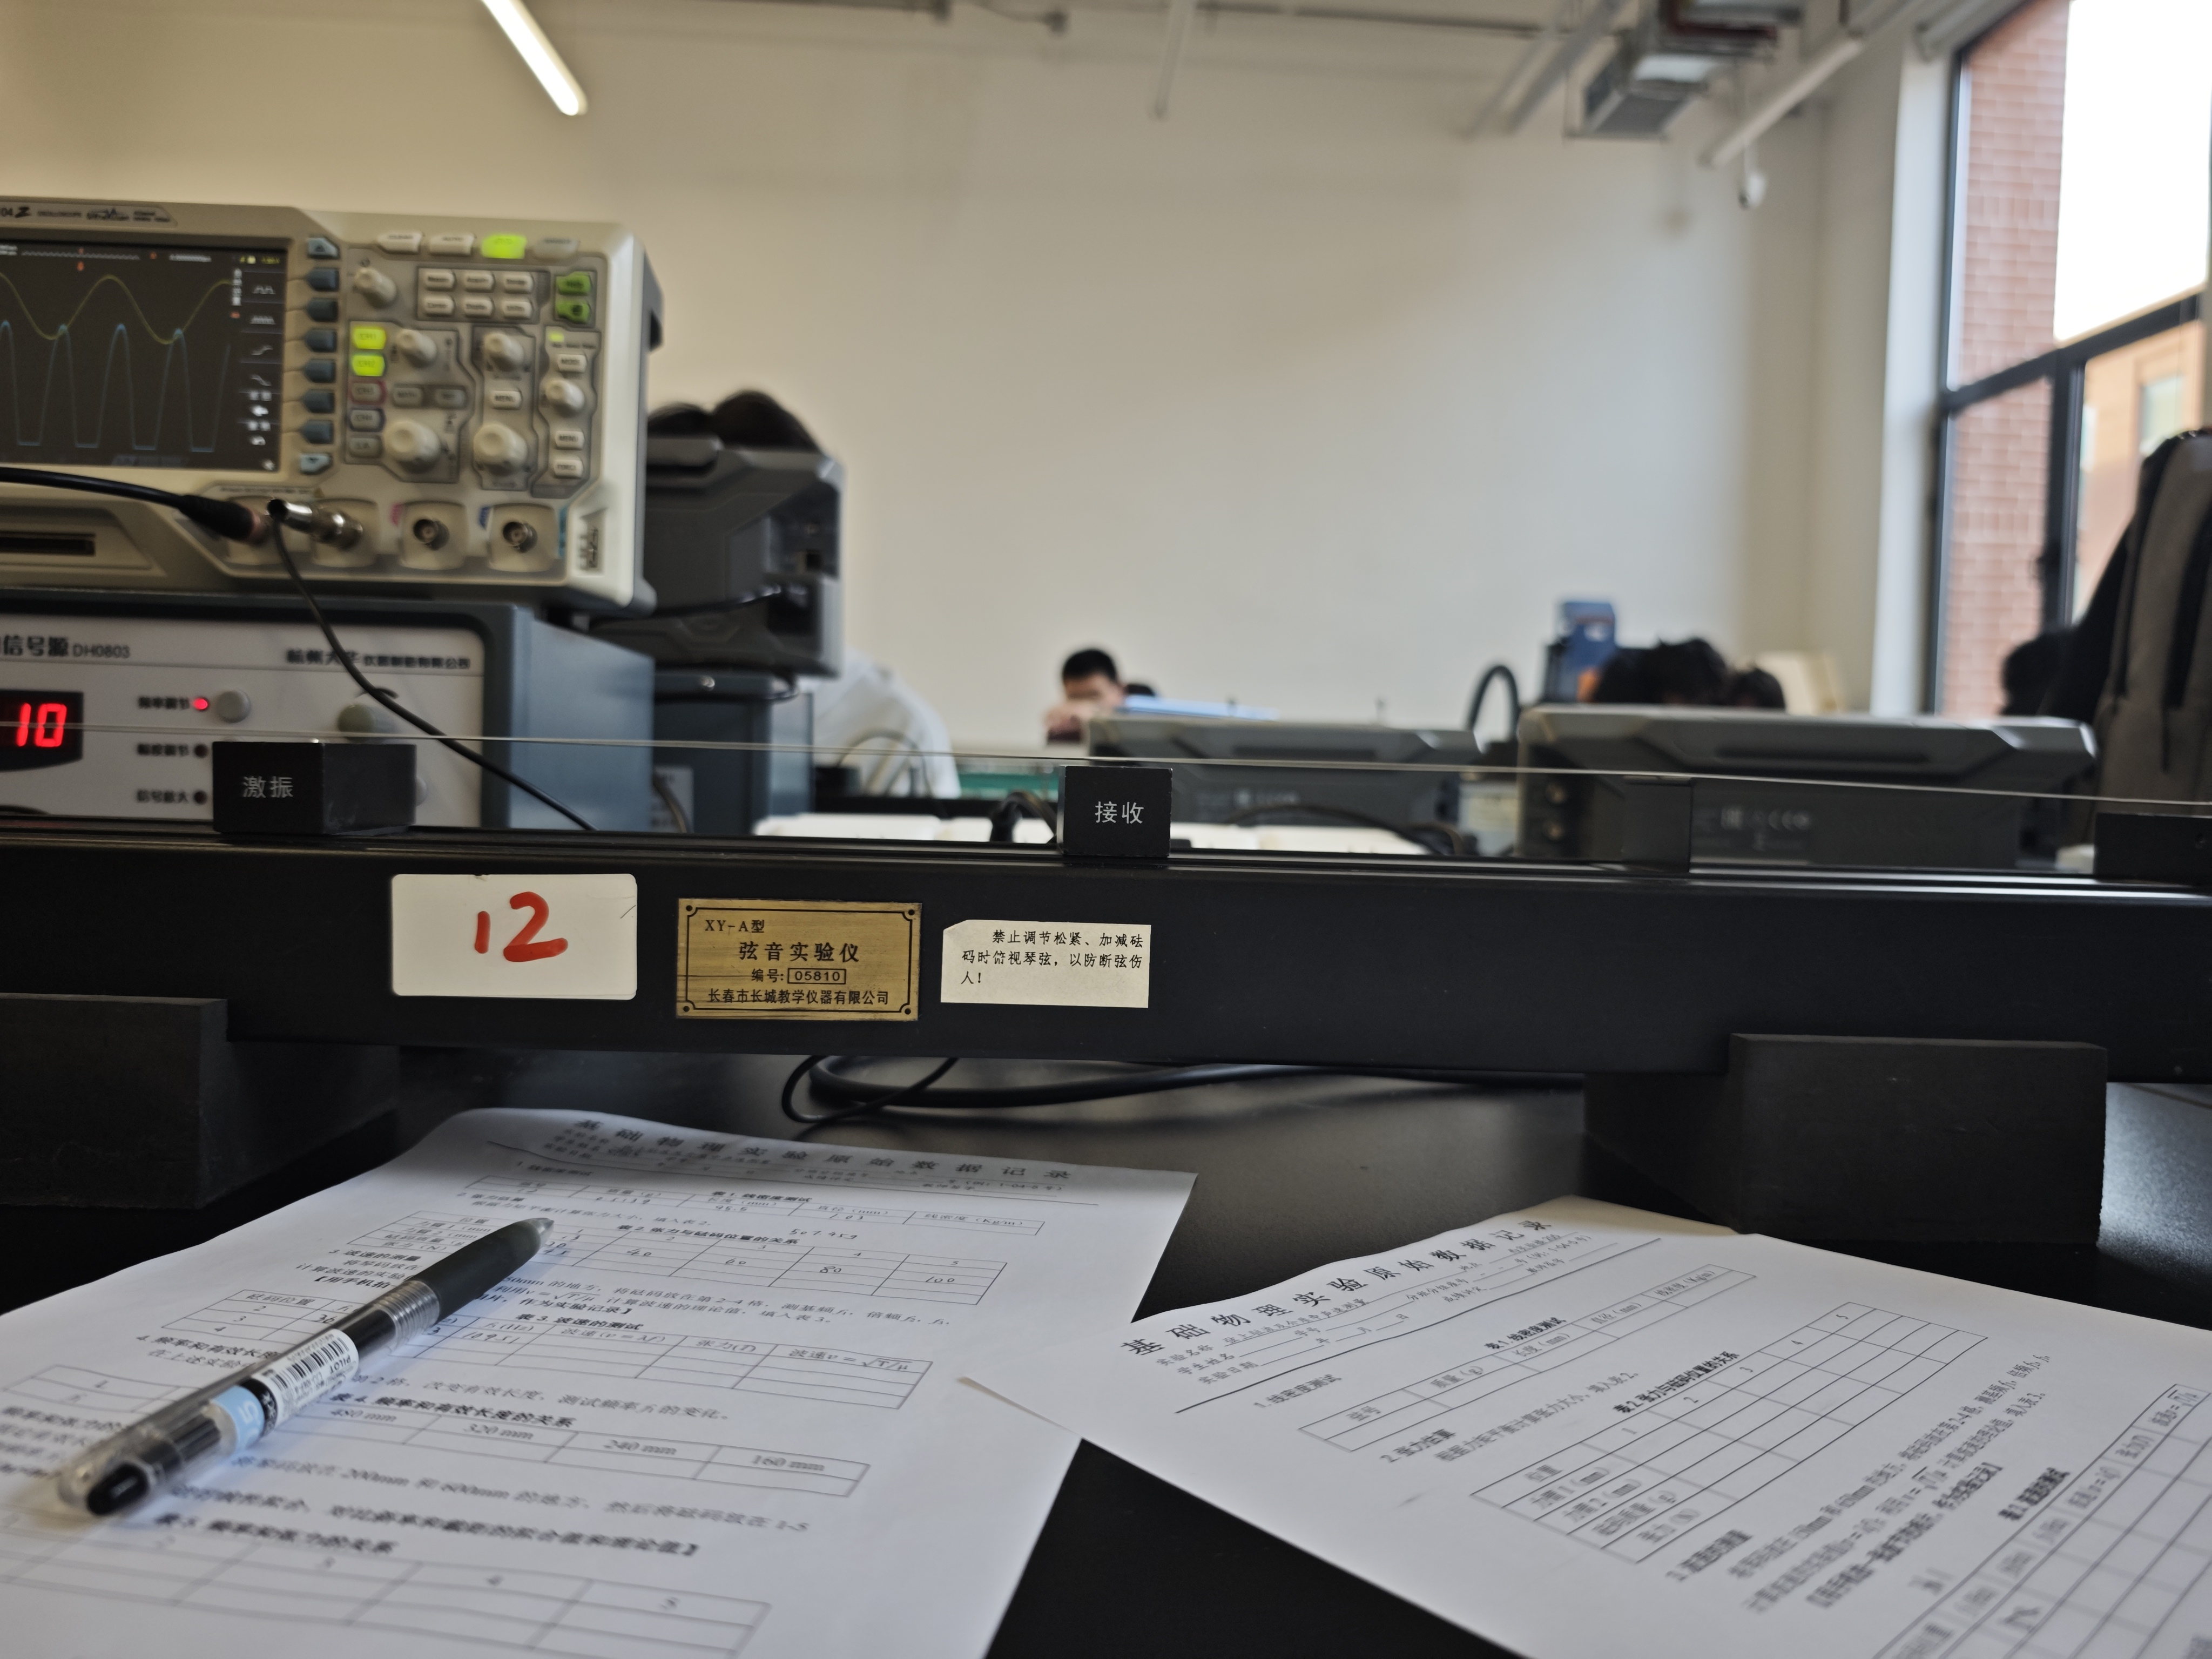
\includegraphics[width=\textwidth]{phe1.jpg}
        \caption{波速测量实验图1}
        \label{fig:phe1}
    \end{subfigure}
    \hfill
    \begin{subfigure}[b]{0.48\textwidth}
        \centering
        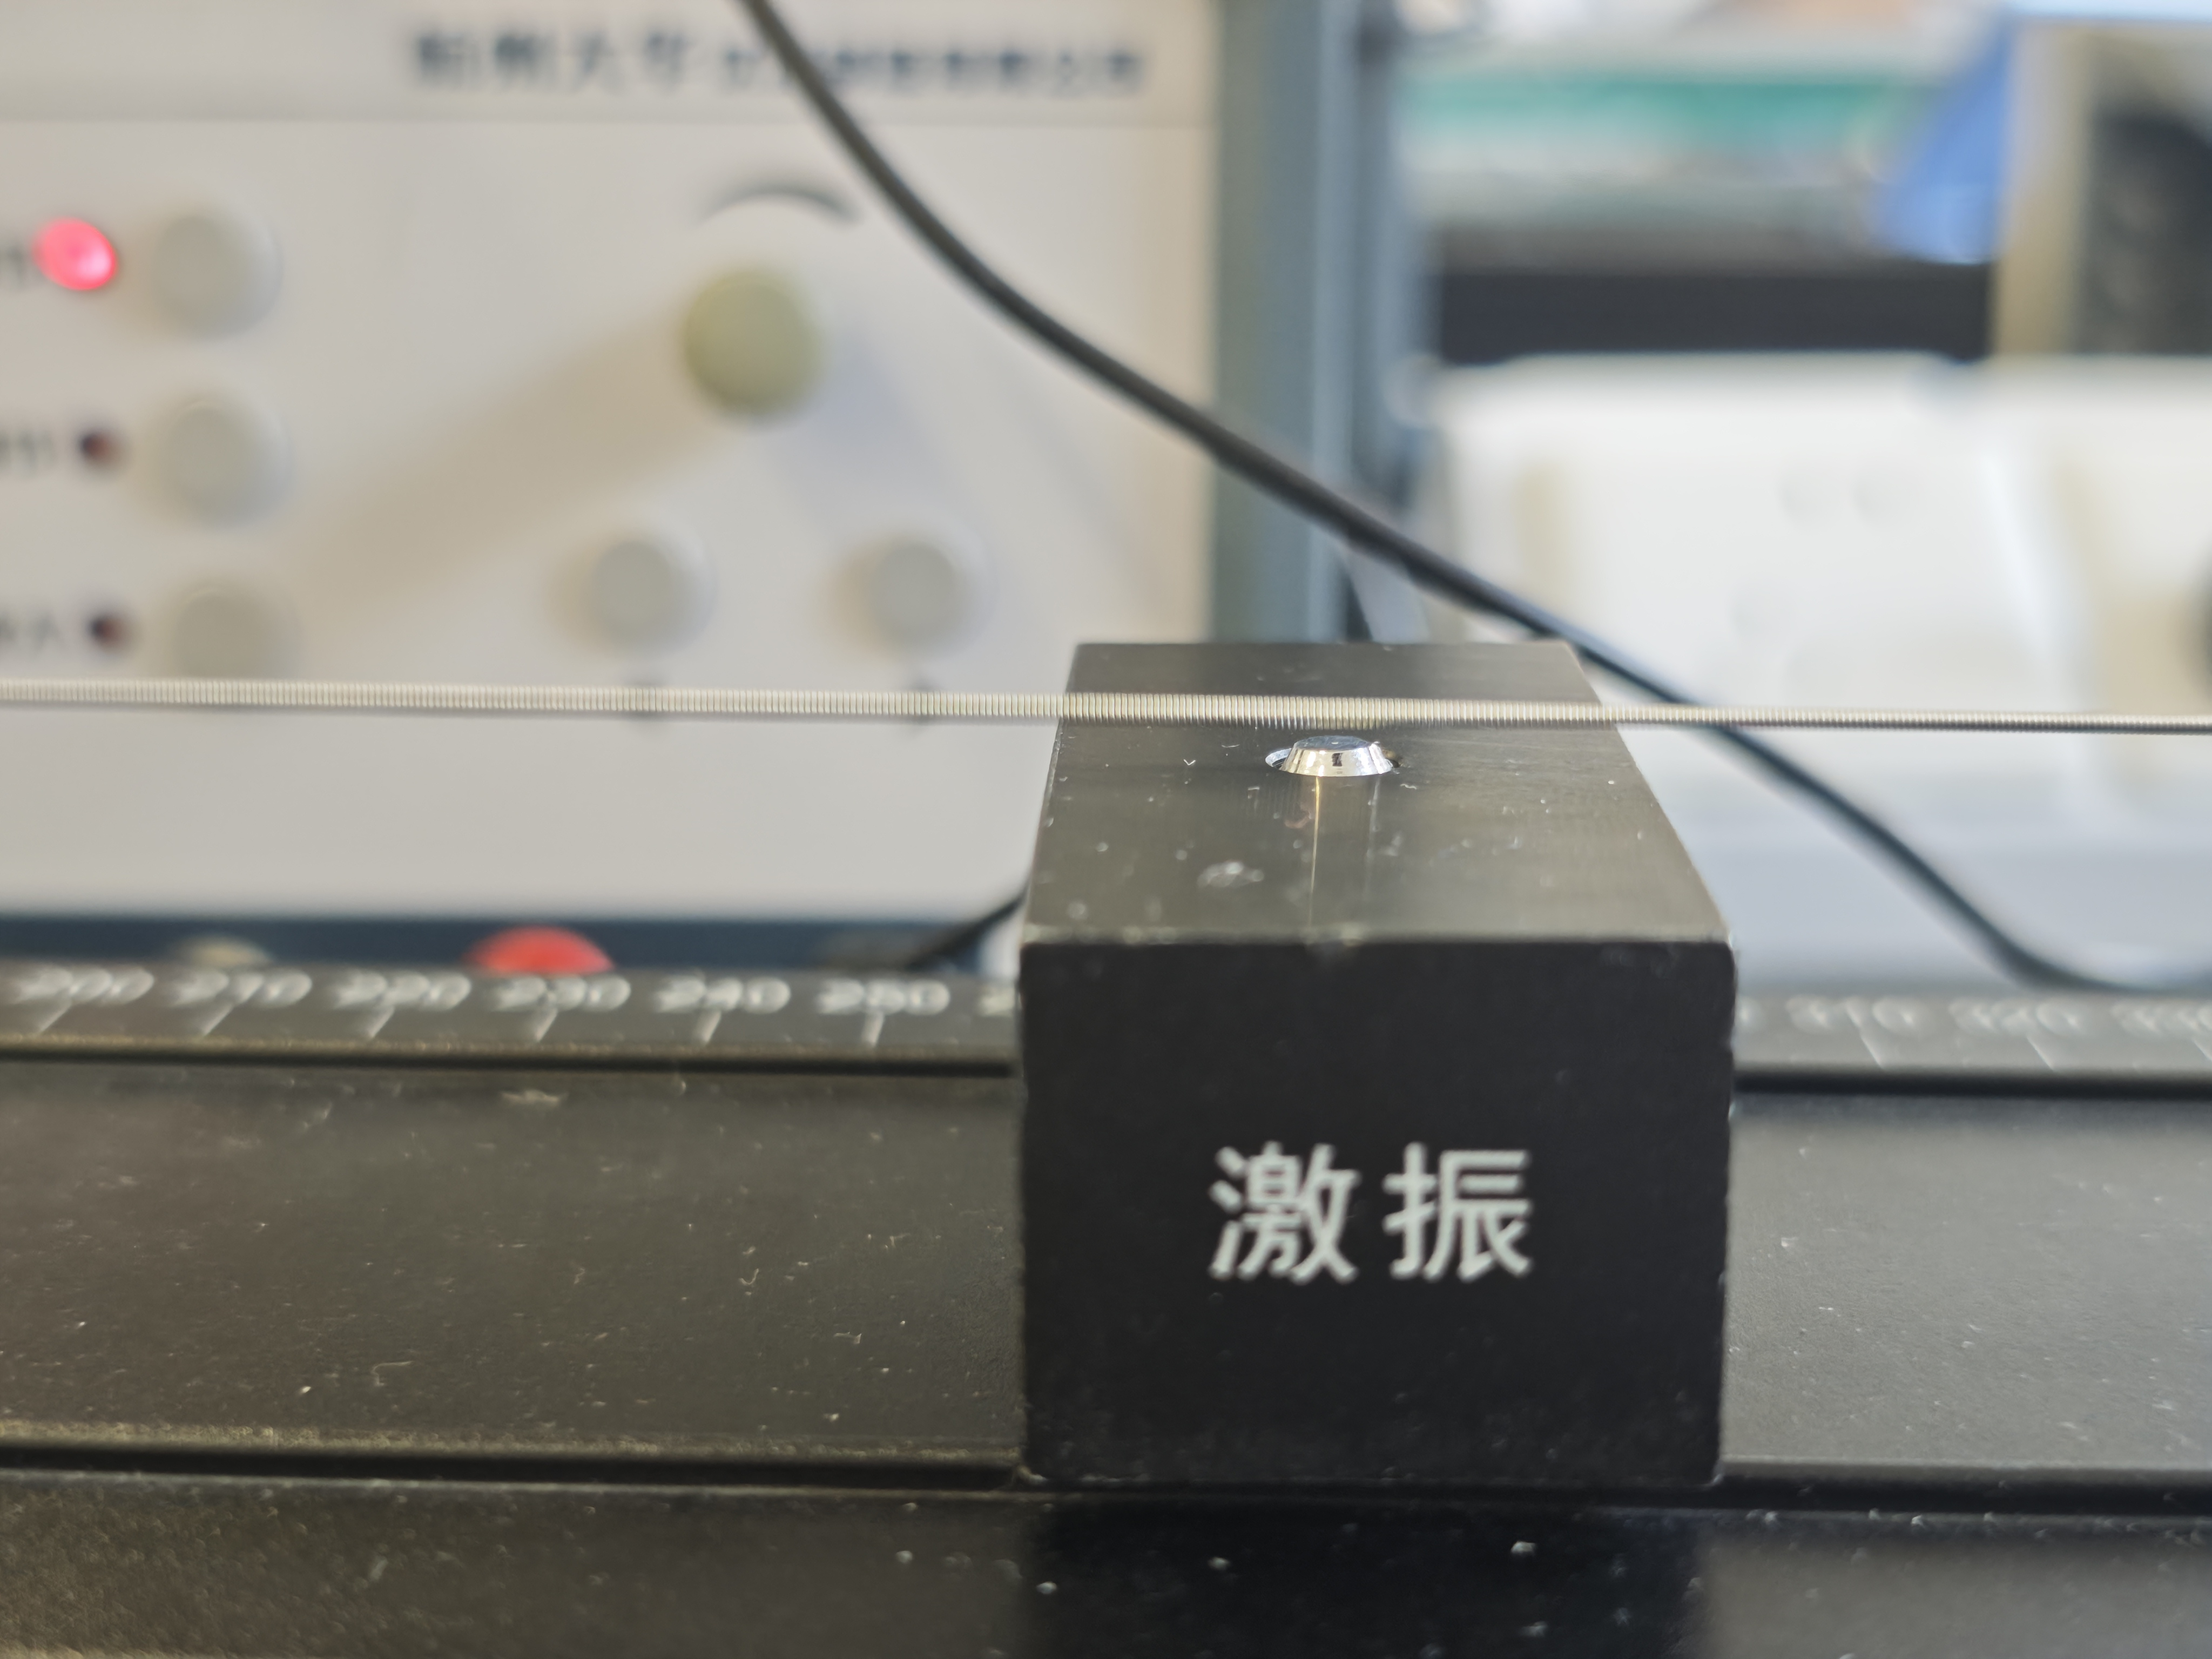
\includegraphics[width=\textwidth]{phe2.jpg}
        \caption{波速测量实验图2}
        \label{fig:phe2}
    \end{subfigure}
    \caption{波速测量实验现场记录}
    \label{fig:wave_measure}
\end{figure}

\begin{table}[h]
    \centering
    \caption{波速的测试}
    \label{tab:2}
    \begin{tabular}{ccccccc}
        \toprule
        砝码位置 & $f_1$ (Hz) & $f_2$ (Hz) & $f_3$ (Hz) & 波速 ($v = \lambda f$) & 张力 ($T$) & 波速 $v = \sqrt{T/\mu}$ \\
        \midrule
        2 & 36.16 & 72.13 & 109.51 & 36.24 & 15.30 & 53.33 \\
        3 & 43.3 & 86.3 & 129.9 & 43.25 & 22.95 & 65.31 \\
        4 & 48.28 & 96.51 & 144.95 & 48.28 & 30.61 & 75.43 \\
        \bottomrule
    \end{tabular}
\end{table}

\subsection{频率和有效长度的关系}

在上述实验中，砝码放在第 2 格，改变有效长度，测试频率 $f_1$ 的变化。

\begin{table}[h]
    \centering
    \caption{频率和有效长度的关系}
    \label{tab:freq_length}
    \begin{tabular}{cccccc}
        \toprule
        L (m) & 0.640 & 0.480 & 0.320 & 0.240 & 0.160 \\
        \midrule
        $1/L$ (m$^{-1}$) & 1.56 & 2.08 & 3.13 & 4.17 & 6.25 \\
        $f_1$ (Hz) & 26.53 & 39.1 & 58.02 & 75.22 & 110.02 \\
        \bottomrule
    \end{tabular}
\end{table}

\textbf{数据分析：}

根据驻波频率公式 $f = \frac{v}{2L}$，当弦线张力和线密度不变时，频率 $f$ 与有效长度 $L$ 成反比，即 $f$ 与 $1/L$ 成正比。

为了验证这一关系，我们将上述数据 $f_1$ 对 $1/L$ 作图并进行线性拟合。

设拟合方程为 $f = A \cdot (1/L) + B$。利用最小二乘法对数据进行线性拟合，得到拟合结果：
$$ f = 17.53 \cdot (1/L) + 1.52 $$
相关系数 $R^2 = 0.997$。

从拟合结果可以看出，$f$ 与 $1/L$ 具有良好的线性关系，说明实验结果符合理论预期。

根据拟合斜率 $k = 17.53$，我们可以推算出波速的实验值：
$$ v_{\text{exp}} = 2k = 35.06 \, \text{m/s} $$

对比之前的波速测量结果，我们可以发现该值与之前的测量值（$36.24$ m/s）较为接近，但与理论计算值（$53.33$ m/s）存在较大差异。这可能是由于实验过程中张力的实际值并没有达到预期的 15.30 N，或者在该有效长度变化实验中，实际使用的张力较小（例如砝码位置可能在第 1 格，对应的张力约为 7.65 N，此时理论波速 $v = \sqrt{7.65/0.00538} \approx 37.7$ m/s，与实验值非常吻合）。


\subsection{频率和张力的关系}

固定有效长度 $L=400\,\text{mm}$，将琴码放在 $200\,\text{mm}$ 和 $600\,\text{mm}$ 的地方，然后将砝码放在 1-5 格时，测频率 $f_1$。

\begin{figure}[H]
    \centering
    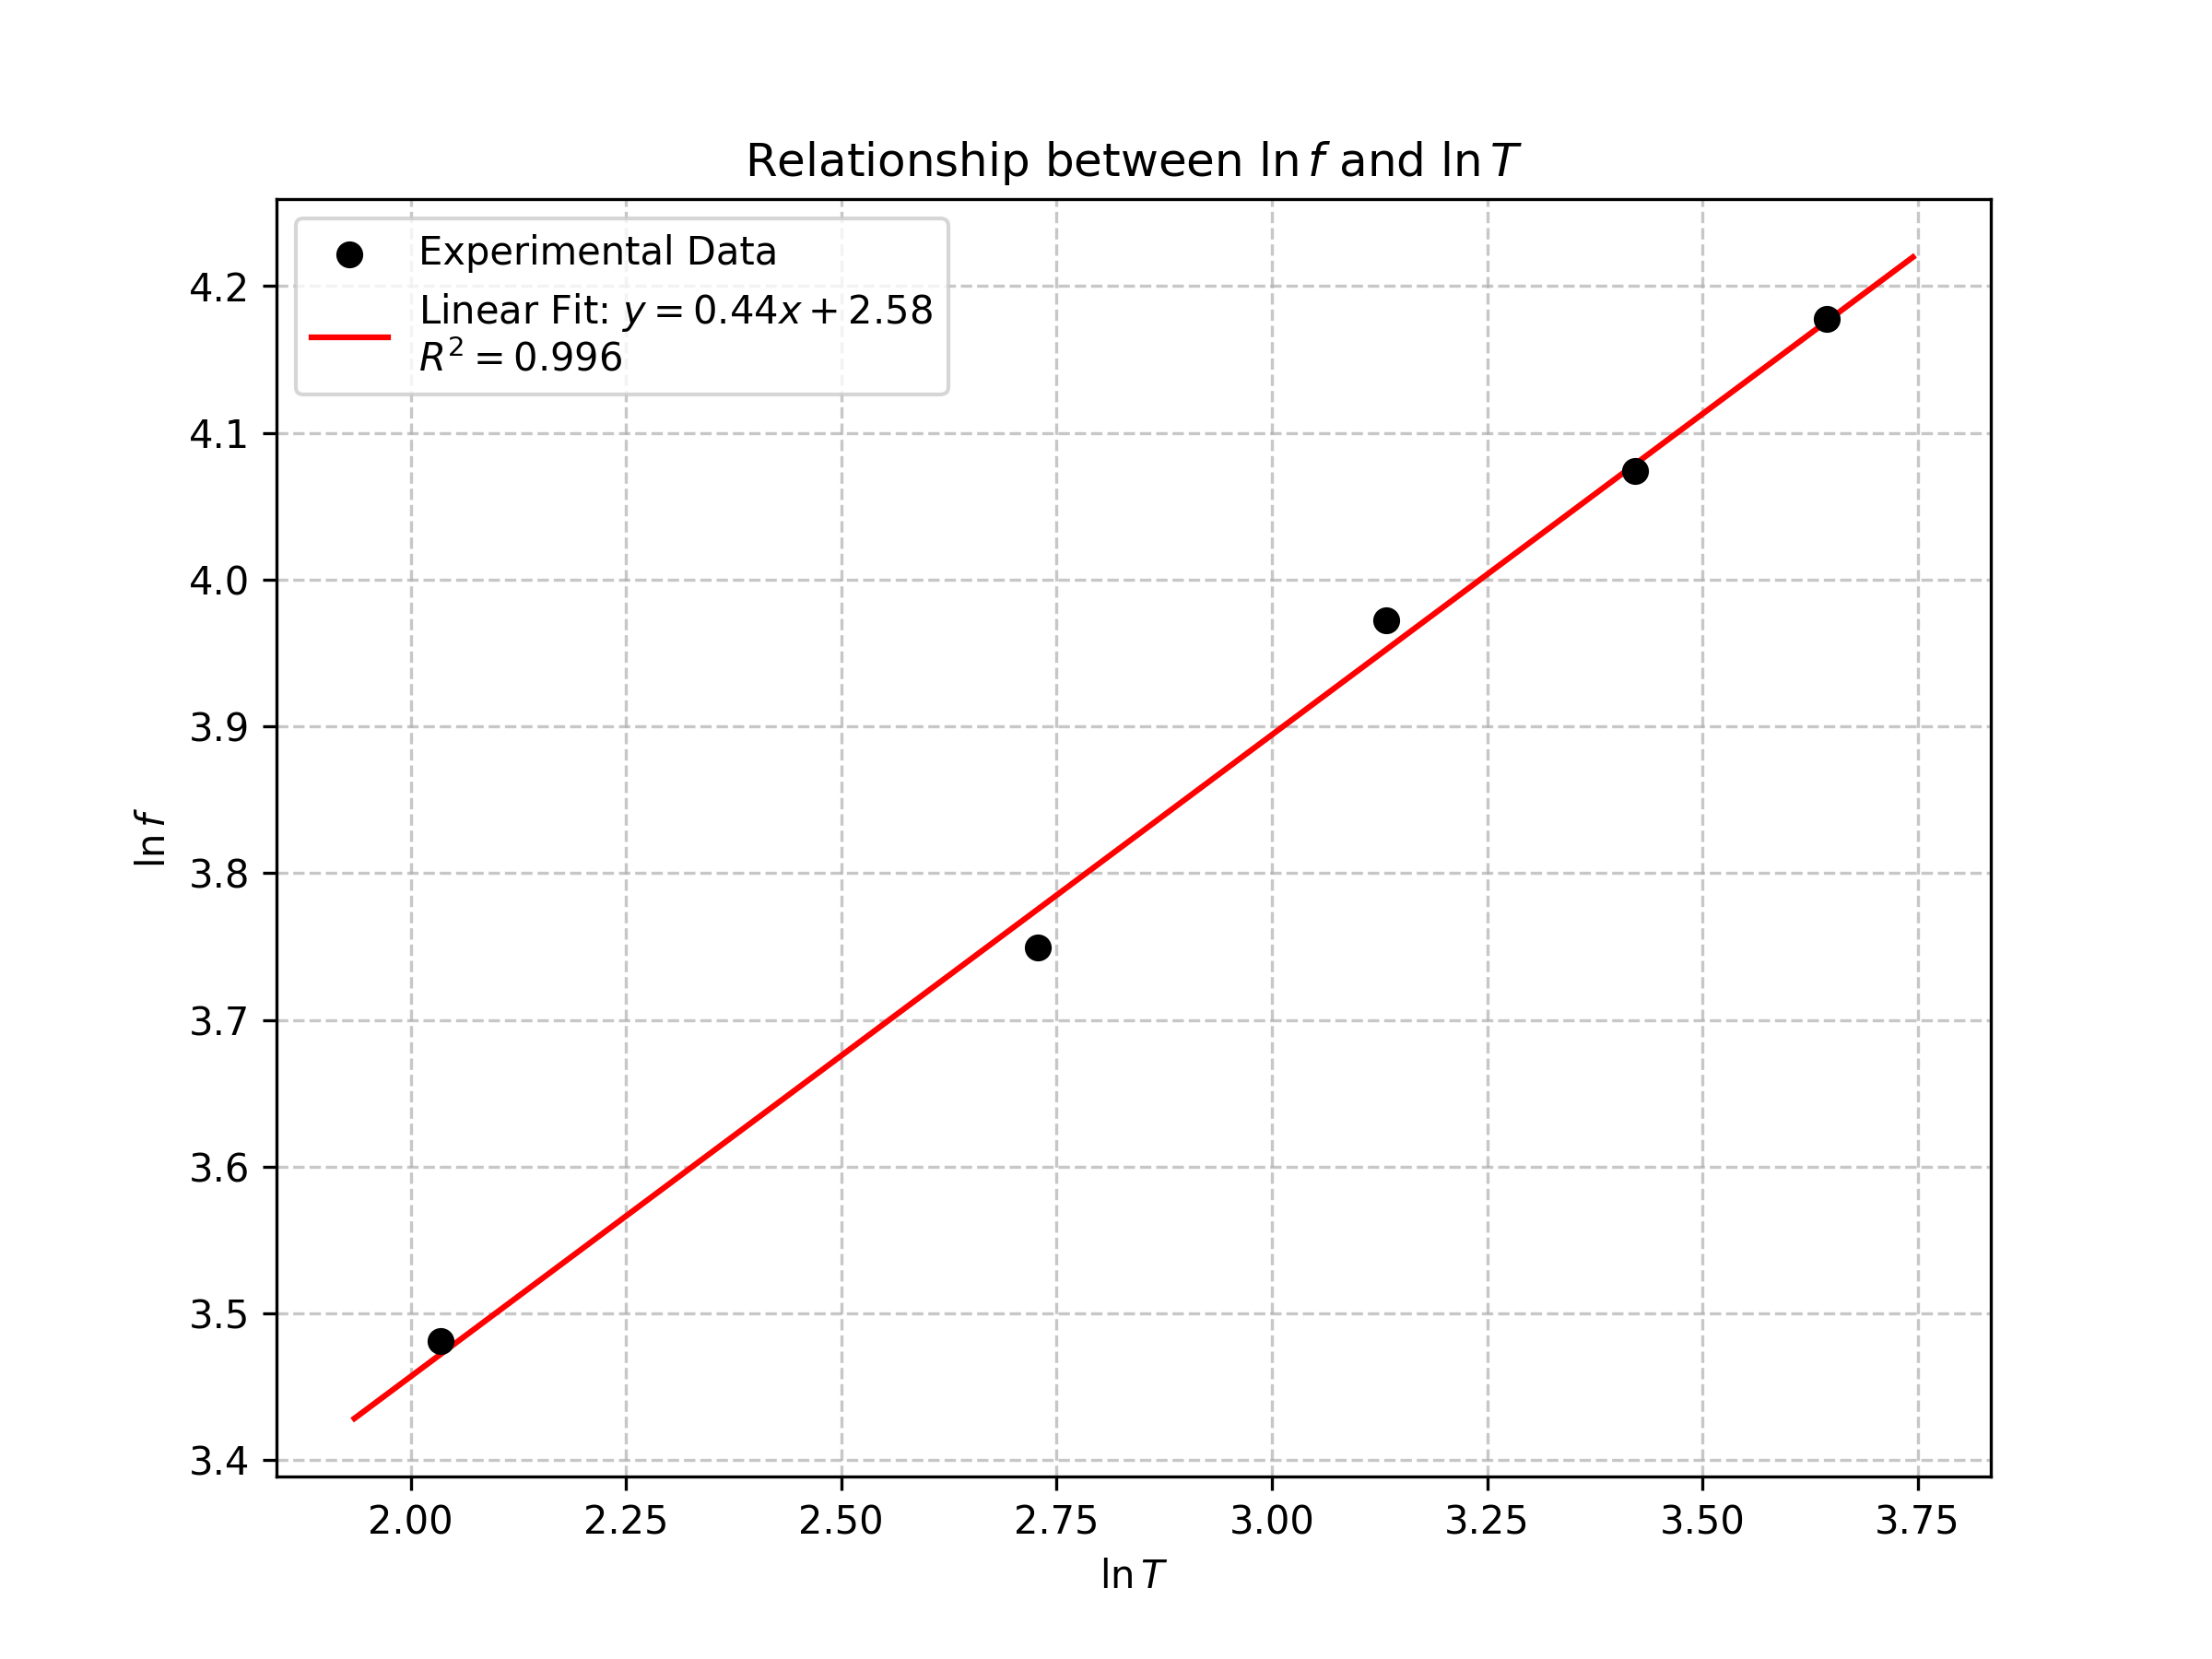
\includegraphics[width=0.7\textwidth]{lnf_lnT_plot.png}
    \caption{$\ln f - \ln T$ 关系曲线及线性拟合}
    \label{fig:lnf_lnT}
\end{figure}

为了验证 $f \propto \sqrt{T}$ 的关系（即 $\ln f = \frac{1}{2} \ln T + C$），我们将张力 $T$ 和频率 $f_1$ 取对数，数据整理如下表：

\begin{table}[h]
    \centering
    \caption{频率和张力的关系（含对数数据）}
    \label{tab:freq_tension}
    \begin{tabular}{cccccc}
        \toprule
        位置 & 1 & 2 & 3 & 4 & 5 \\
        \midrule
        $T$ (N) & 7.65 & 15.30 & 22.95 & 30.61 & 38.26 \\
        $\ln T$ & 2.03 & 2.73 & 3.13 & 3.42 & 3.64 \\
        $f_1$ (Hz) & 32.5 & 42.5 & 53.1 & 58.8 & 65.2 \\
        $\ln f_1$ & 3.48 & 3.75 & 3.97 & 4.07 & 4.18 \\
        \bottomrule
    \end{tabular}
\end{table}

\textbf{数据分析：}

根据弦振动公式 $f = \frac{1}{2L}\sqrt{\frac{T}{\mu}}$，两边取对数得：
\begin{equation}
    \ln f = \frac{1}{2} \ln T - \frac{1}{2} \ln \mu - \ln(2L)
\end{equation}
理论上，$\ln f - \ln T$ 图像应为一条直线，其斜率 $k_{theo} = 0.5$。
代入已知常数 $\mu = 0.00538 \, \text{kg/m}$ 和 $L = 0.400 \, \text{m}$，可得理论截距：
$$ b_{theo} = - \frac{1}{2} \ln(0.00538) - \ln(0.8) \approx 2.84 $$

利用最小二乘法对实验数据进行线性拟合，设拟合方程为 $\ln f = k \ln T + b$。
拟合结果如下：
\begin{itemize}
    \item 实验斜率 $k_{exp} \approx 0.44$
    \item 实验截距 $b_{exp} \approx 2.58$
    \item 相关系数 $R^2 \approx 0.996$
\end{itemize}

\textbf{结果讨论：}
实验数据的线性相关度很高（$R^2$ 接近 1），说明频率与张力的平方根确实成正比关系。
实验斜率 $0.44$ 略小于理论值 $0.5$，截距 $2.58$ 也小于理论值 $2.84$。这可能是由于弦线的弯曲刚度等非理想因素的影响，或者张力的实际值因摩擦等原因略小于计算值。

\section{思考题}
\begin{enumerate}
    \item 调节振动源上的振动频率和振幅大小后对弦线振动会产生什么影响？
    \item 如何来确定弦线上的波节点位置？
    \item 在弦线上出现驻波的条件是什么？在实验中为什么要把弦线的振动调到驻波现在最稳定、最显著的状态？
    \item 在弹奏弦线乐器时，发出声音的音调与弦线的长度、粗细、松紧程度有什么关系？为什么？
    \item 若样品弦线与装置上的弦线直径略有差别，请判断是否需要修正，如何进行？
    \item 对于某一共振频率，增大或减少频率的调节过程中，振幅最大的频率位置往往不同，如何解释这一现象？
\end{enumerate}
\subsection{频率和线密度的关系}

固定有效长度 $L = 400 \text{ mm}$，将琴码放在 $200 \text{ mm}$ 和 $600 \text{ mm}$ 的地方，将砝码放在第 3 格。测不同粗细琴弦的基频 $f_1$，也可以共享其它同学的实验数据。

\subsubsection{实验数据记录}

\begin{table}[h]
    \centering
    \caption{频率与线密度的关系数据记录表}
    \label{tab:freq_density}
    \begin{tabular}{cccccc}
        \toprule
        弦号 & 2 & 12 & 6 & 3 & 8 \\ 
        \midrule
        直径 (mm) & 0.818 & 1.03 & 1.06 & 0.670 & 0.680 \\ 
        $\mu$ (kg/m) & 0.0034 & 0.0054 & 0.0056 & 0.0021 & 0.0022 \\ 
        $f_1$ (Hz) & 64.4 & 53.1 & 49.14 & 77.8 & 78.2 \\ 
        \bottomrule
    \end{tabular}
\end{table}

\subsubsection{理论模型与拟合分析}

根据弦振动理论，基频 $f_1$ 与线密度 $\mu$ 的关系为：
$$f_1 = \frac{1}{2L} \sqrt{\frac{T}{\mu}}$$

两边取对数得：
$$\ln f_1 = \ln \left( \frac{\sqrt{T}}{2L} \right) - \frac{1}{2} \ln \mu$$

由此可知，$\ln f_1$ 与 $\ln \mu$ 理论上呈线性关系，理论斜率为 $-0.5$。

\begin{figure}[H]
    \centering
    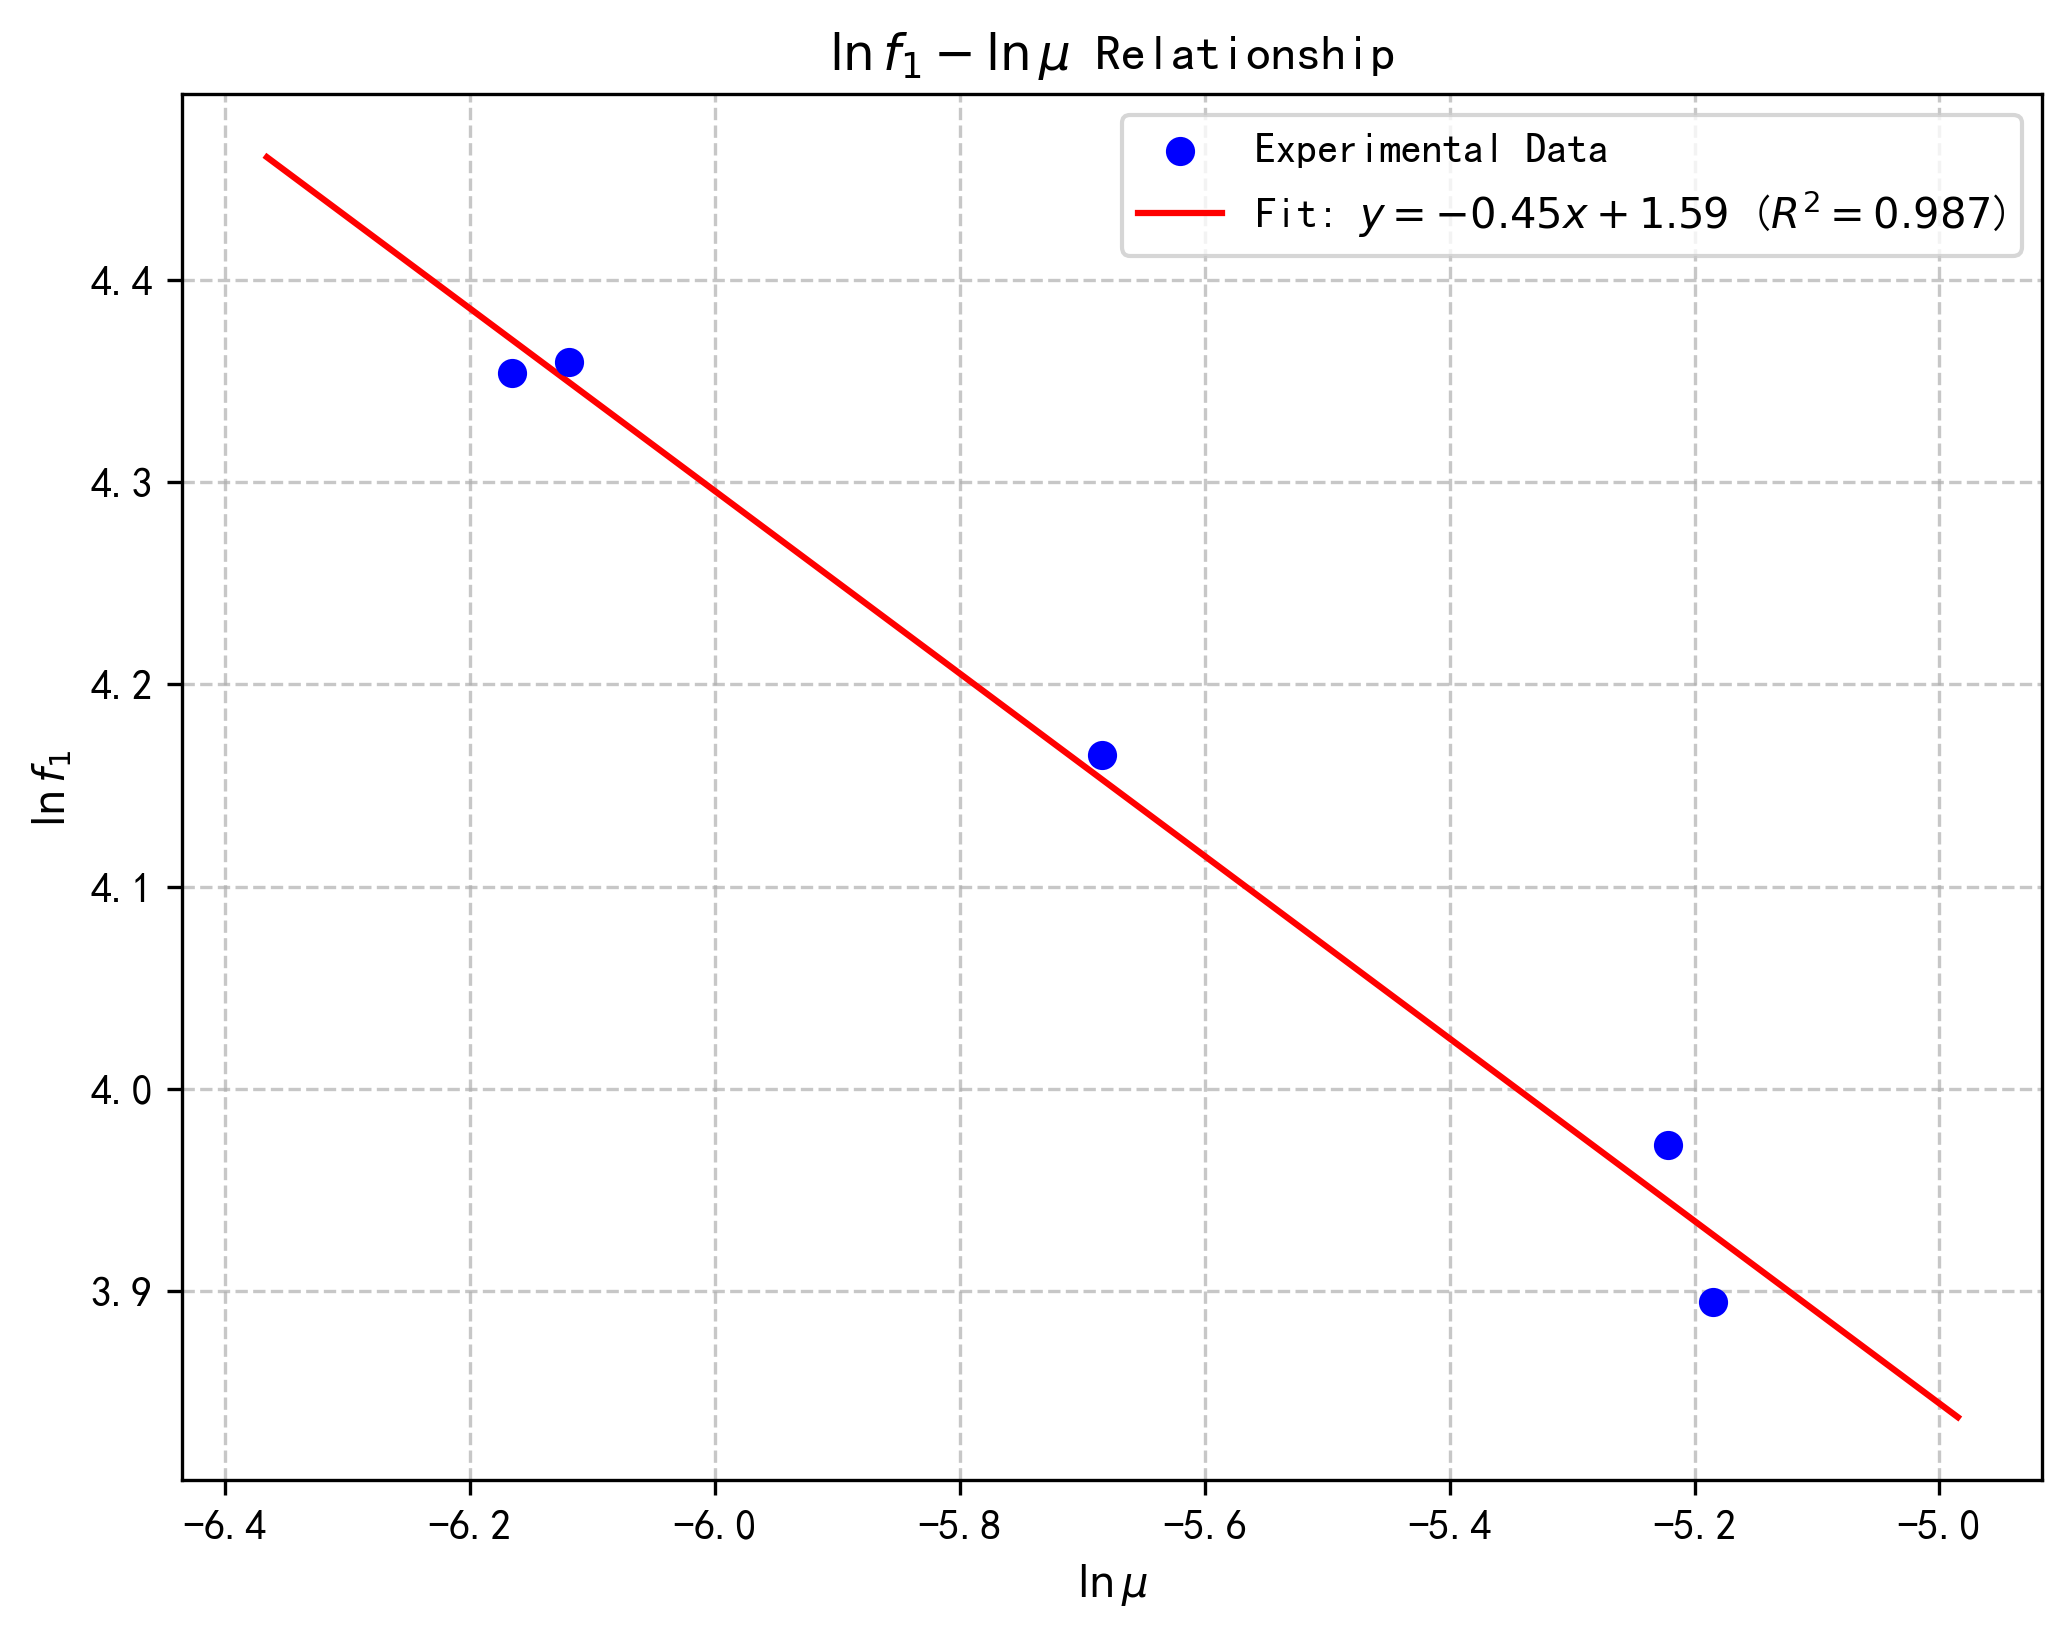
\includegraphics[width=0.7\textwidth]{lnf_lnmu_plot.png}
    \caption{$\ln f_1 - \ln \mu$ 关系曲线及线性拟合}
    \label{fig:lnf_lnmu}
\end{figure}

为了验证上述关系，我们将频率 $f_1$ 和线密度 $\mu$ 取对数，利用最小二乘法进行线性拟合。

设拟合方程为 $\ln f_1 = k \ln \mu + b$。拟合结果如下：
\begin{itemize}
    \item 实验斜率 $k_{exp} \approx -0.45$
    \item 实验截距 $b_{exp} \approx 1.59$
    \item 相关系数 $R^2 \approx 0.99$
\end{itemize}

\textbf{结果讨论：}

理论上，斜率应为 $-0.5$。截距的理论值（$T=22.95\,\text{N}, L=0.400\,\text{m}$）为：
$$ b_{theo} = \ln \left( \frac{\sqrt{22.95}}{2 \times 0.400} \right) \approx 1.79 $$

对比实验结果与理论值，线性拟合的相关系数较高，说明 $\ln f_1$ 与 $\ln \mu$ 确实呈现良好的线性关系。实验斜率 $-0.45$ 与理论值 $-0.5$ 接近但略小，截距 $1.59$ 也略小于理论值 $1.79$。这可能是由于弦线的实际线密度与标称值存在偏差，或者弦线的刚度效应在细弦和粗弦上的表现不同导致的误差。

\newpage

\part{测定介质中的声速}


\section{实验目的}
\begin{enumerate}
    \item 利用驻波法测定波长；
    \item 利用相位法测定波长；
    \item 计算超声波在空气中和水中的传播速率。
\end{enumerate}
\begin{figure}[H]
    \centering
    
\includegraphics[width=0.8\textwidth]{fig7}
    \caption{SW-2 声速测量仪}
    \label{fig:fig7}
\end{figure}

\section{实验仪器与用具}
SW-2型声速测量仪，信号发生器，示波器。SW-2型声速测量仪如图\ref{fig:fig7}所示。

% [图片位置: 图7 SW-2 声速测量仪]

\begin{figure}[H]
    \centering
    
\includegraphics[width=0.8\textwidth]{fig8}
    \caption{纵波的传播情况 (a)介质中粒子处于平衡位置的情况 (b)声波中介质粒子偏离平衡位置的情况}
    \label{fig:fig8}
\end{figure}。

\section{实验原理}
空气中的声波是一种纵波。纵波是指质点振动方向平行于传播方向的波。与之对应的是横波，即质点振动方向垂直于波传播方向的波。声波在空气中传播时只能发生压缩与膨胀，空气质点的振动方向与声波的传播方向一致，所以空气中的声波是纵波（如图\ref{fig:fig8}）。

% [图片位置: 图8 纵波的传播情况 (a)介质中粒子处于平衡位置的情况 (b)声波中介质粒子偏离平衡位置的情况]

\subsection{利用驻波法测声速}
将信号发生器输出的正弦电压信号接到超声发射换能器上，超声发射换能器通过电声转换，将电压信号变为超声波，以超声波形式发射出去。接收换能器通过声电转换，将声波信号变为电压信号，送入示波器。

由声波传输理论可知，从发射换能器发出一定频率的平面声波，经过介质传播到达接收换能器。如果接收面和发生面严格平行，即入射波在接收面上垂直反射，入射波和反射波相互干涉形成驻波。此时，两换能器之间的距离恰好等于其声波半波长的整数倍，在声驻波中，波腹处声压最小，波节处声压最大。接收换能器的反射界面处为波节，声压效果最大。所以，可以从接收换能器端面声压的变化来判断超声波是否形成驻波。

转动鼓轮，改变两只换能器间的距离，在一系列特定的距离上，将会出现稳定的驻波，记录下出现最大电压数值时标尺上的刻度，相邻两次最大值对应的刻度值之差即为半波长。根据公式 $v=\lambda f$，频率 $f$ 已知，根据上述方法可以求出波长 $\lambda$，就可以算出超声波的传播速度 $v$。

\subsection{利用相位法测声速}
将发射波和接收波同时输入示波器，并且以X-Y模式显示，两波的频率相同，相位不同。当接收点和发射点的距离变化等于一个波长时，相位差正好是 $2\pi$。
\begin{figure}[H]
    \centering
    
\includegraphics[width=0.6\textwidth]{fig9}
    \caption{频率相同、相位不同时的李萨如图形}
    \label{fig:fig9}
\end{figure}
实验时，通过改变发射器和接收器之间的距离，观察相位的变化，当相位改变 $\pi$，相应距离的改变量即为半波长。根据公式 $v=\lambda f$，求出波速。

相位变化时，李萨如图形如图\ref{fig:fig9}所示。

% [图片位置: 图9 频率相同、相位不同时的李萨如图形]

\subsection{声速的理论值}
利用声速在空气中的理论公式可以计算空气中声速的理论值。
\begin{equation}
    v=v_{0}\sqrt{\frac{T}{T_{0}}}=v_{0}\sqrt{1+\frac{t}{273.15}}
\end{equation}
其中：$T=(t+273.15)K$，$v_{0}=331.45$ m/s，为0℃时的声速，$t$ 为摄氏温度。

\section{实验内容}
\begin{enumerate}
    \item 利用驻波法和相位法测超声波在空气中的波速。
    \item 利用驻波法或相位法测超声波在水中的波速。
    \item 利用逐差法处理实验数据。
\end{enumerate}

\section{实验数据}
\subsection{空气中超声波波速的测试}

% 实验基本参数
已知声源频率 $f = 40\,\text{kHz}$，室温 $t = 27.1\,^\circ\text{C}$，理论声速 $v_{\text{理论}} = 347.50\,\text{m/s}$。

\subsubsection{实验数据记录}

\begin{table}[h]
    \centering
    \caption{空气中超声波波速测试数据表}
    \label{tab:air_speed}
    \begin{tabular}{ccccc}
    \toprule
    $i$ & 驻波法 $L_i$ (mm) & $\Delta L_{i, i+5}$ (mm) & 相位法 $L_i$ (mm) & $\Delta L_{i, i+5}$ (mm) \\ 
    \midrule
    1  & 40.18 & 22.52 & 41.09 & 22.16 \\ 
    2  & 44.47 & 22.73 & 45.48 & 21.91 \\ 
    3  & 49.50 & 22.13 & 49.84 & 22.06 \\ 
    4  & 53.13 & 22.88 & 54.23 & 22.12 \\ 
    5  & 58.28 & 22.22 & 58.75 & 22.07 \\ 
    6  & 62.70 & - & 63.25 & - \\ 
    7  & 67.20 & - & 67.39 & - \\ 
    8  & 71.63 & - & 71.90 & - \\ 
    9  & 76.01 & - & 76.35 & - \\ 
    10 & 80.50 & - & 80.82 & - \\ 
    \midrule
    \multicolumn{2}{c}{测量结果: $\bar{\lambda}=9.00\,\text{mm}, v = 359.94\,\text{m/s}$} & \multicolumn{3}{c}{测量结果: $\bar{\lambda}=8.83\,\text{mm}, v = 353.02\,\text{m/s}$} \\ 
    \bottomrule
    \end{tabular}
\end{table}

\subsubsection{数据处理说明}

根据逐差法计算波长 $\lambda$。
对于驻波法和相位法，分别计算5组间隔为5的差值 $\Delta L = L_{i+5} - L_i$。
平均波长 $\bar{\lambda}$ 由下式给出：
\[ \bar{\lambda} = \frac{2}{5} \overline{\Delta L} \]
计算得：
\begin{itemize}
    \item 驻波法：$\overline{\Delta L} = 22.50\,\text{mm}$，$\bar{\lambda} = 9.00\,\text{mm}$
    \item 相位法：$\overline{\Delta L} = 22.06\,\text{mm}$，$\bar{\lambda} = 8.83\,\text{mm}$
\end{itemize}

再结合频率 $f = 40\,\text{kHz}$ 计算波速 $v = f \cdot \bar{\lambda}$：
\begin{itemize}
    \item 驻波法测得波速：$v_1 = 359.94\,\text{m/s}$
    \item 相位法测得波速：$v_2 = 353.02\,\text{m/s}$
\end{itemize}

与理论值 $v_{\text{理论}} = 347.50\,\text{m/s}$ 相比，相对误差分别为：
\[ E_1 = \left| \frac{359.94 - 347.50}{347.50} \right| \times 100\% \approx 3.58\% \]
\[ E_2 = \left| \frac{353.02 - 347.50}{347.50} \right| \times 100\% \approx 1.59\% \]

\subsection{水中超声波波速的测试}

方法：相位法，频率 $f = 1.7\,\text{MHz}$，室温 $t = 26.9\,^\circ\text{C}$。

\subsubsection{实验数据记录（表\ref{tab:water_speed}）}

\begin{table}[h]
    \centering
    \caption{水中超声波波速测试数据表}
    \label{tab:water_speed}
    \begin{tabular}{cccc}
    \toprule
    $i$ & 刻度值 $L_i$ (mm) & $\Delta L_{i, i+5}$ (mm) & $\lambda_i = \frac{2}{5}\Delta L_{i, i+5}$ (mm) \\ 
    \midrule
    1  & 40.01 & 2.21 & 0.8840 \\ 
    2  & 40.58 & 2.10 & 0.8400 \\ 
    3  & 40.87 & 2.24 & 0.8960 \\ 
    4  & 41.55 & 2.07 & 0.8280 \\ 
    5  & 41.82 & 2.48 & 0.9920 \\ 
    6  & 42.22 & - & - \\ 
    7  & 42.68 & - & - \\ 
    8  & 43.11 & - & - \\ 
    9  & 43.62 & - & - \\ 
    10 & 44.30 & - & - \\ 
    \midrule
    \multicolumn{4}{c}{测量结果: $\bar{\lambda}=0.8880\,\text{mm}, v = 1509.60\,\text{m/s}$} \\ 
    \bottomrule
    \end{tabular}
\end{table}

\subsubsection{结果与分析}

结合表中测得的 $\lambda$ 序列，由 $v = f \cdot \bar{\lambda}$ 计算水中声速实验值：
\[ \bar{\lambda} = \frac{1}{5} \sum_{i=1}^{5} \lambda_i = 0.8880\,\text{mm} \]
\[ v_{\text{exp}} = f \cdot \bar{\lambda} = 1.7 \times 10^6 \times 0.8880 \times 10^{-3} = 1509.60\,\text{m/s} \]

理论声速值（考虑温度修正）：
根据水的声速经验公式（Lubbers and Graaff公式近似），在 $t = 26.9^\circ\text{C}$ 时，纯水中的声速约为：
\[ v_{\text{theo}} \approx 1502.36\,\text{m/s} \]

与实验值相比，相对误差为：
\[ E = \left| \frac{1509.60 - 1502.36}{1502.36} \right| \times 100\% \approx 0.48\% \]

可见实验结果与理论值吻合较好，误差较小。误差可能来源于读数误差（如第5组数据偏差较大）或水温测量的准确性。

\section{预习报告和原始记录}

\begin{figure}[H]
    \centering
    
\includegraphics[width=0.95\textwidth]{record_pre.jpg}
    \caption{预习报告}
\end{figure}

\begin{figure}[H]
    \centering
    
\includegraphics[width=0.95\textwidth]{record1.jpg}
    \caption{原始记录1}
\end{figure}

\begin{figure}[H]
    \centering
    
\includegraphics[width=0.95\textwidth]{record2.jpg}
    \caption{原始记录2}
\end{figure}

\end{document}